\documentclass[final]{beamer}
\usepackage[scale=1.24]{beamerposter}
\usepackage{graphicx}
\usepackage{lipsum}
\usepackage[font=small]{caption}
\newlength{\sepwid}
\newlength{\colwidside}
\newlength{\colwidmiddle}
\setlength{\paperwidth}{56in}
\setlength{\paperheight}{36in}
\setlength{\sepwid}{0.03\paperwidth}
\setlength{\colwidside}{0.25\paperwidth}
\setlength{\colwidmiddle}{0.38\paperwidth}
\setlength{\topmargin}{-0.5in}
%\setlength{\topmargin}{1in}
\usetheme{confposter}
\usepackage{exscale}

\makeatletter
\let\@@magyar@captionfix\relax
\makeatother

\usecaptiontemplate{
\small 
\structure{\insertcaptionname~\insertcaptionnumber:}
\insertcaption}
% (see beamerthemeconfposter.sty to change color definitions)
\setbeamercolor{block title}{fg=ngreen,bg=white}
\setbeamercolor{block body}{fg=black,bg=white}
\setbeamercolor{block alerted title}{fg=white,bg=dblue!70}
\setbeamercolor{block alerted body}{fg=black,bg=dblue!10}
% Making titles
\title{Spatiotemporal Modeling of Voting in North Carolina} 
\author{Marschall Furman, Andrew Giffin, Matt Miller}
\institute{North Carolina State University}


% Poster is divided into three columns, and columns divided into 3,1 and 2 blocks (the map in the centre of the poster is not a block, just a graphic). The code in the white region is LaTeX language, and the code in the gray regions is R language.

\usepackage{Sweave}
\begin{document} 
\Sconcordance{concordance:poster.tex:poster.Rnw:%
1 32 1 1 42 3 1 1 0 21 1 1 7 30 1 1 7 23 1 1 6 15 0 1 2 59 1 1 8 28 1}

\begin{frame}[t]
\begin{columns}[t]
\begin{column}{\sepwid}\end{column}
\begin{column}{\colwidside}


\begin{block}{Project Goal}
   The 13 voting districts in North Carolina have repeatedly been struck down
   by the courts for (illegal) racial gerrymandering; and the state has
   received national attention for its highly (legally) politically
   gerrymandered districts -- which have been accused of guarding
   the majority party (Republican) seats, despite voting fluctuations.

   \vspace{.2in}

   This project examines the publically available
   highly local precinct-level voting and
   demographic data which feed into the district voting data, using a
   spatial areal-data model.
\end{block}
\vskip2ex

\begin{block}{The Data}  
  \begin{itemize}
    \item Examining voting data for US House of Representatives races,
      for years 2002, 2004, \ldots, 2018. 
    \item Currently 2,704 precincts. Due to boundary changes over time, and
      missing data, we model a subset of 2,045 of these precincts.
    \item The publically available election data includes:
      precinct-level vote counts (the response); as well as
      precinct-level demographic data on age, race, and sex (the predictors).   
    \item \begin{center}\Large{covariate plots?}\end{center}
  % \begin{figure}
  %   \center
  %     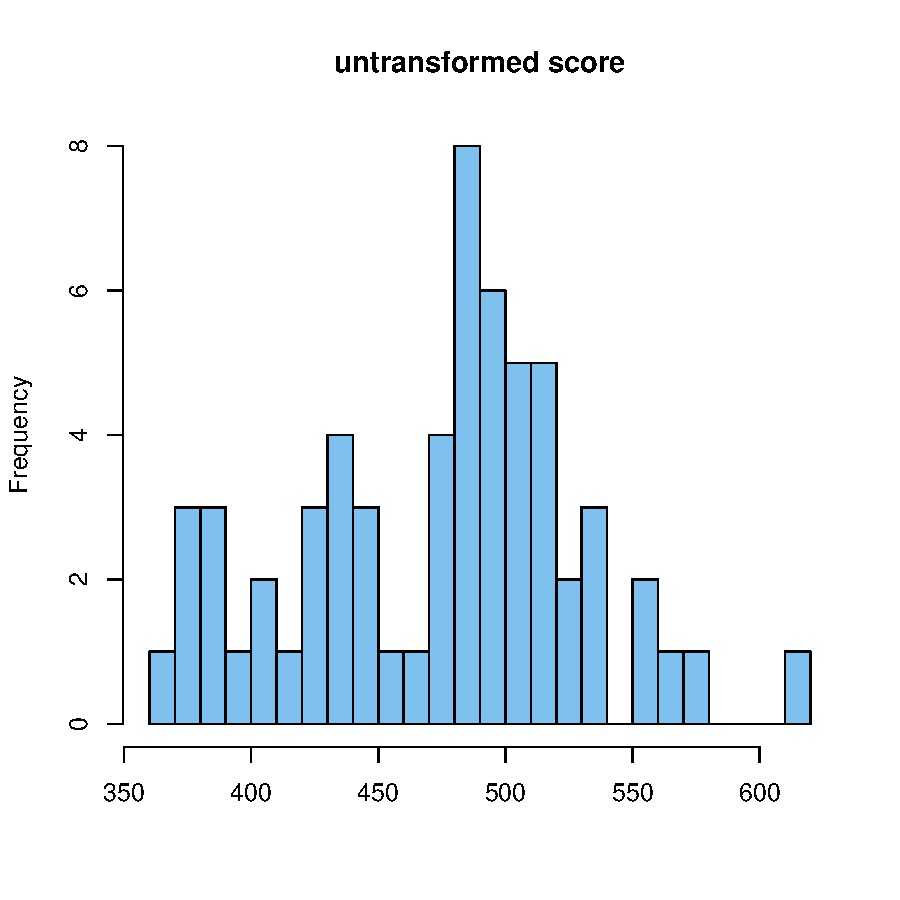
\includegraphics[width=.35\colwidside]{poster-t1.pdf}
  %     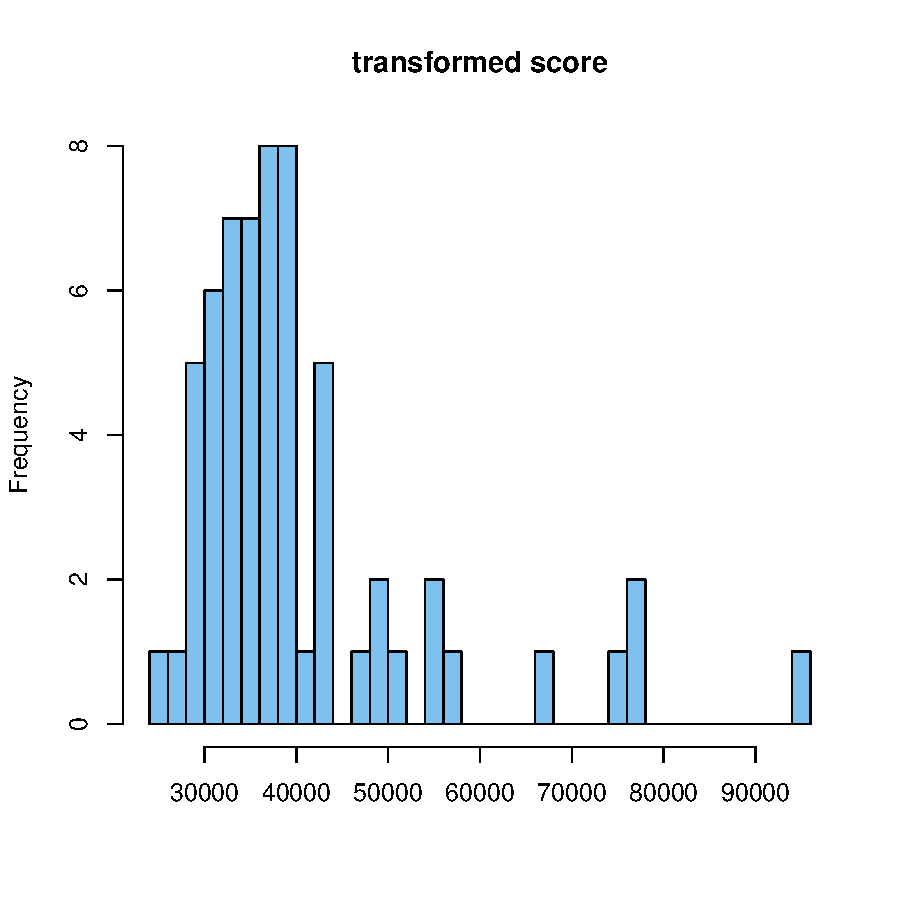
\includegraphics[width=.35\colwidside]{poster-t2.pdf}
  %   \caption{Histograms of the data, the untransformed data is
  %     displayed on the left and the transformed data is on the right,
  %     see below for details about the transformation.}
  %   \end{figure}
    \item Because this project relied of many different publically available
      datasets, a substantial amount of work was put into cleaning and
      standardizing the data. As a result of data irregularites, there
      are a number of caveats that we include with out data:
      \begin{itemize}
        \item A substantial number of precincts were not reported for
          each year -- either due to the precincts having changed over
          time, changing of precinct naming schemes, or missing
          data. All such precincts were excluded from our model.
        \item Because absentee and early voting was not often reported
          at the individual precinct level, we excluded all absentee
          and early voting voters counts (usually $\sim 3\%$ of the votes)
          which could introduce bias.
        \item Within each precinct, there were often covariates that
          had missing data. Our estimates simply summed over the
          available covariates.
        \item One particular modeling nuisance was the occurrence of
          several elections with \emph{unopposed} candidates
          (resulting in $\theta_{kt}$ at exactly 0 or 1.) 
        \end{itemize}
      \item Lastly, we used the full Binomial model, rather than the
          common normal approximation, because the normal 
          approximation is ineffective for probabilities close to 0 or
          1 -- which is the case with a substantial number of our
          observed precincts.
    \end{itemize}
\end{block}
  
\vskip2ex
\begin{block}{Modeling Decisions}
\begin{enumerate}
\item Type of data
  \begin{itemize}
    \item I think binomial is the correct choice now
    \item We are still modeling the logit of the proportion, but it is within the Binomial model
  \end{itemize}
\item Type of Spatiotemporal CAR model
    \begin{itemize}
    \item Many options in the package
    \item I think ST.CARlocalised() is promising because it might detect anomalies that could be linked to election fraud – neat point to talk about on the poster
    \item 
  \end{itemize}
\item How to calculate adjacency matrix
    \begin{itemize}
      \item Package allows in most cases to have adjacency matrices with non-binary value
      \item This kind of makes interpretation weird
      \item I think we should have a binary adjacency matrix, but we
        need to decide if there’s a threshold for centroid-centroid
        distance that we consider ``adjacent'' or if we’re actually
        doing true adjacency
  \end{itemize}
\item How to predict
    \begin{itemize}
    \item $\text{expit}(\mathbf{x}_{kt}^T \pmb{\hat{\beta}}+ \psi_{kt})$
    \item Use estimated demographic values in $x$
    \item Not sure what to do for estimating the spatio-temporal
      effects. Regression and extrapolations?
  \end{itemize}
\end{enumerate}
%   \begin{itemize}
%     \item Since data are averages over countries -- we first transformed them to
%     to satisfy the homoscedasticity assumption:
%   \end{itemize}
% % Equations for the weights:
%   \[
%     y = X\beta + \epsilon \quad \rightarrow \quad W^{\frac{1}{2}}y = W^{\frac{1}{2}}X\beta + W^{\frac{1}{2}}\epsilon \quad \mbox{,      \quad where}
%   \]
% % Matrix for the weights:
%   \[
%   W^{\frac{1}{2}} = \left[ \begin{array}{ccc}
%   \sqrt{n_1} & \cdots & 0 \\
%   \vdots & \ddots & \vdots \\
%   0 & \cdots &  \sqrt{n_{62}}\\
%   \end{array} \right], \quad n_j = \mbox{number of students in country~} j
%   \]

% % Creating the scatter matrices in block 3
%   \begin{figure} 
%     \center 
%       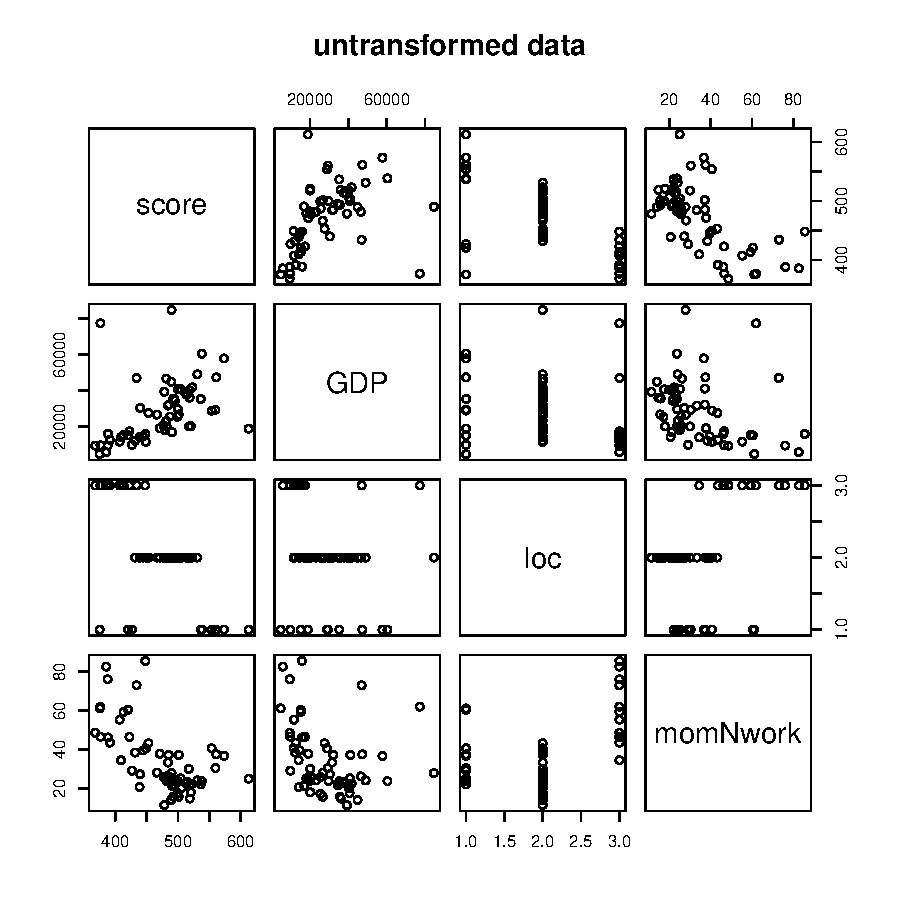
\includegraphics[width=0.4\colwidside]{poster-p1.pdf} 
%       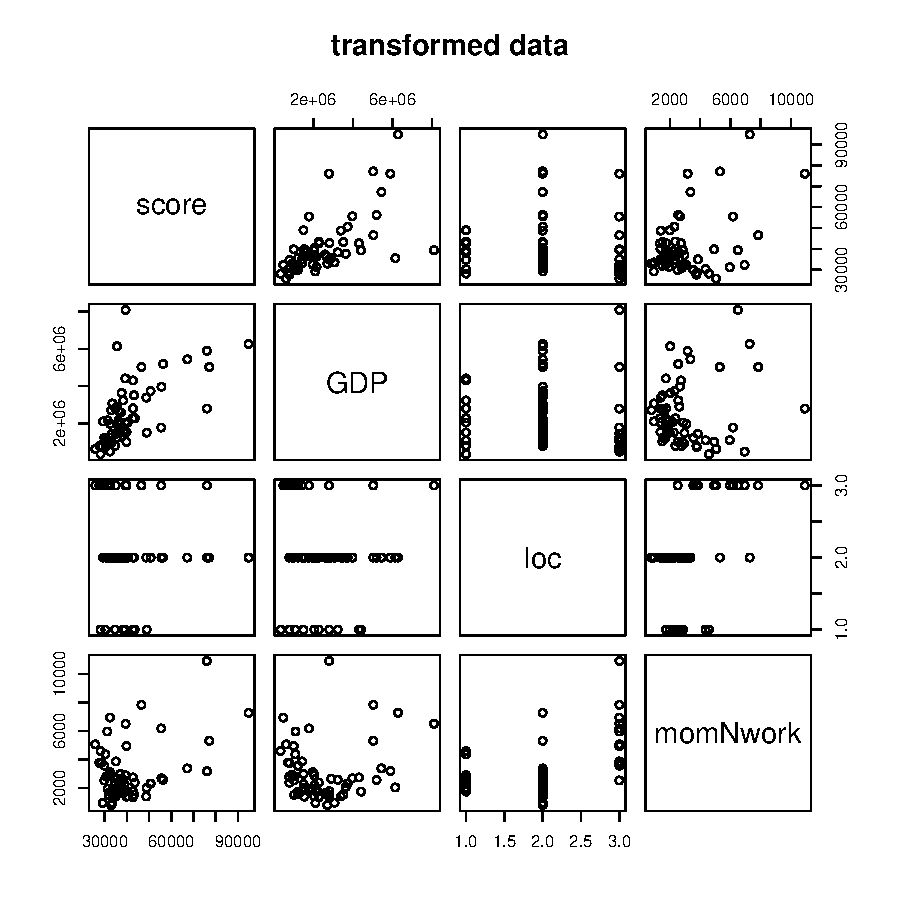
\includegraphics[width=0.4\colwidside]{poster-p2.pdf} 
%   \caption{Scatter matrices of some of the untransformed variables (left) and transformed variables (right). $GDP$ denotes GDP per capita, $loc$ denotes if the country is in the Western, Asian or Other category, and $momNwork$ denotes the average percentage of students in the country who has a mom who is not working.}
%   \end{figure}
\end{block}
  \vskip2ex
\end{column} \begin{column}{\sepwid}\end{column}





% Starting column 2
\begin{column}{\colwidmiddle}
  % \begin{figure}[ht]
  %     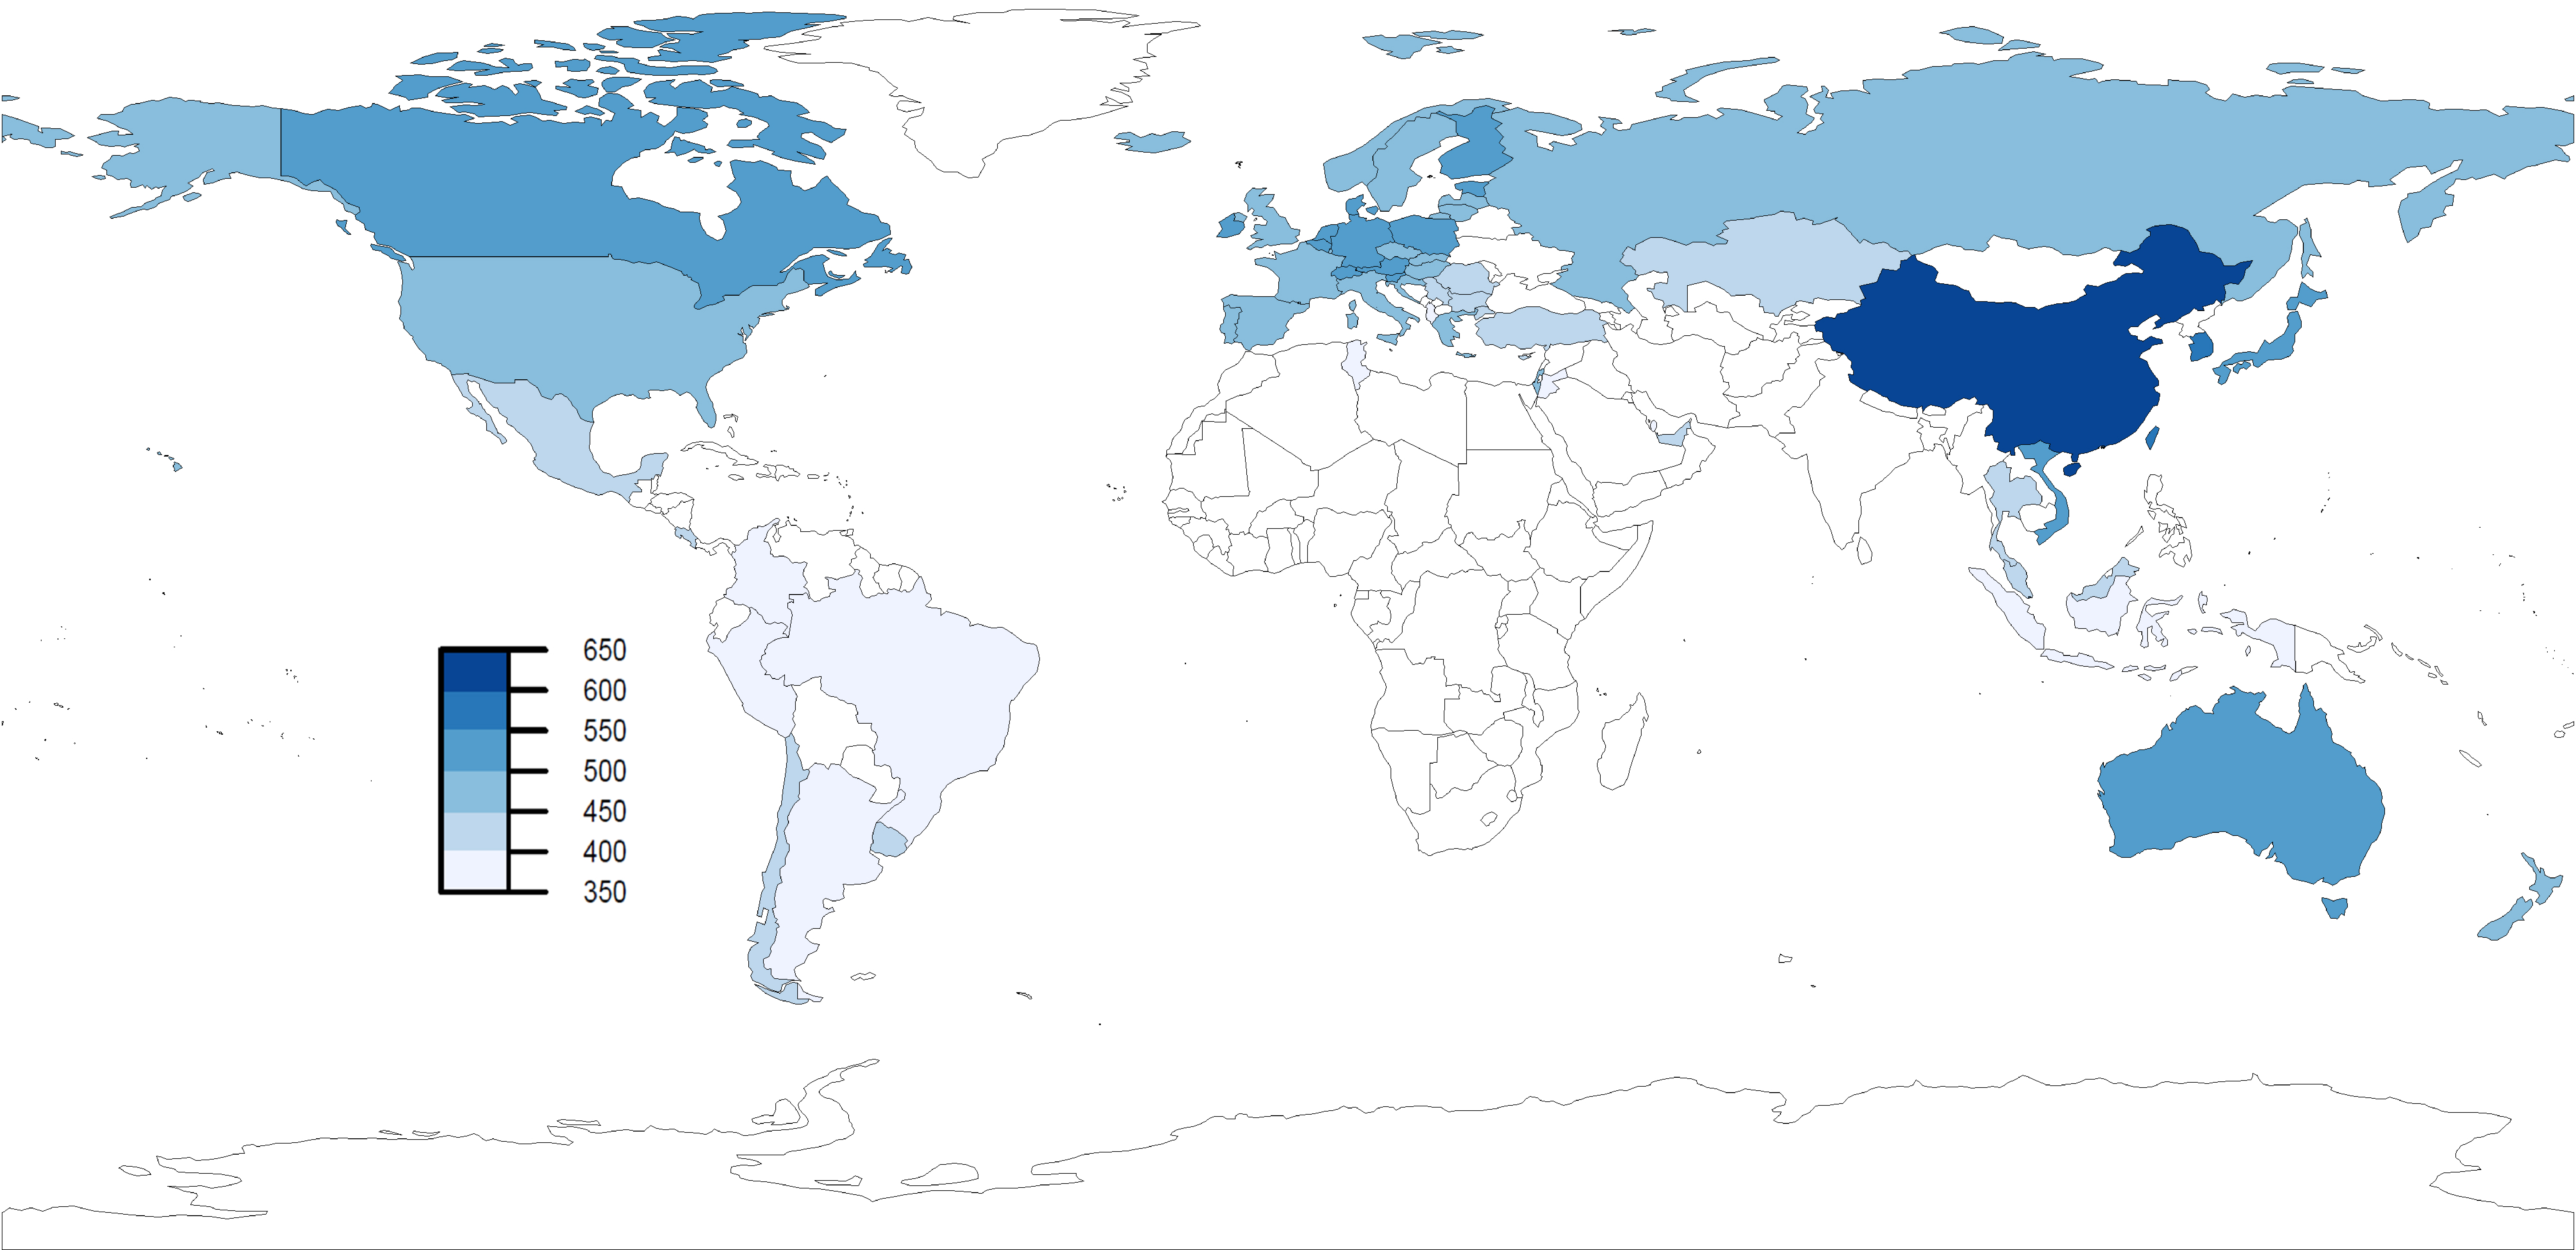
\includegraphics[width=.9\colwidmiddle]{REALscore_WM_LegendE.pdf}
  %   \caption{A map depicting the observed test scores for each country. A dark color represents a high score.}
  % \end{figure}
  % \vskip2ex
 \begin{alertblock}{Spatiotemporal Model}

\vspace{.2in}
   
\textbf{Variables Definitions}
\begin{itemize}
  \item $Y_{kt}$: Number of Democratic votes in precinct $k$ for year
  $t$
  \item $n_{kt}$: Sum of Democratic and Republican votes in precinct
    $k$ for year $t$
  \item $\theta_{kt}$: Relative proportion of Democratic votes in
    precinct $k$ for year $t$
  \item $\mathbf{x_{kt}}$: Vector of covarites in precinct $k$ for
    year $t$
  \item $\psi_{kt}$: Latent component incorporating spatiotemporal
    effects in precinct $k$ for year $t$
\end{itemize}

  \vspace{.5in}

   
\textbf{Model form}

\begin{align*}
  Y_{kt} &\sim \text{Binomial}( n_{kt}, \theta_{kt} ) \\
%  \log \left( \frac{\theta_{kt}}{1 - \theta_{kt}} \right) &=
%  \mathbf{x}_{kt}^\top\mathbf{\beta} + \psi_{kt} \\
    \log \left( \theta_{kt}/(1 - \theta_{kt}) \right) &= \mathbf{x}_{kt}^\top\mathbf{\beta} + \psi_{kt} \\
  \mathbf{\beta} &\sim \text{Normal}(\mathbf{\mu}_{\mathbf{\beta}},
                   \mathbf{\Sigma}_{\mathbf{\beta}})\\
  \psi_{kt} &= \beta_1 + \phi_k + (\alpha +
              \delta_k)\frac{t-\bar{t}}{N} \\
  \phi_k | \pmb{\phi}_{-k}, \mathbf{W} &\sim \text{Normal}\left(
          \frac{\rho_{int} \sum_{j=1}^K  w_{kj}
                                        \phi_j}{\rho_{int}\sum_{j=1}^K
                                        w_{kj} + 1 - \rho_{int}},
          \frac{\tau^2_{int}}{\rho_{int}\sum_{j=1}^K
                                        w_{kj} + 1 -
                                        \rho_{int}}\right)\\
  \delta_k | \pmb{\delta}_{-k}, \mathbf{W} &\sim \text{Normal}\left(
          \frac{\rho_{slo} \sum_{j=1}^K  w_{kj}
                                        \delta_j}{\rho_{slo}\sum_{j=1}^K
                                        w_{kj} + 1 - \rho_{slo}},
          \frac{\tau^2_{int}}{\rho_{slo}\sum_{j=1}^K
                                        w_{kj} + 1 -
                                                \rho_{slo}}\right)\\
  \tau_{int}^2, \tau_{slo}^2 &\sim \text{Inverse Gamma}(1,.01)\\
  \rho_{int}, \rho_{slo} &\sim \text{Uniform}(0,1)\\
  \alpha &\sim \text{Normal}(0, 1000)\\
\end{align*}

\vspace{-.5in}
where $\bar{t} = N^{-1}\sum_{t=1}^N t$ and the linear trend
$(t-\bar{t})/N$ runs over $[-\frac{1}{2}, \frac{1}{2}]$; \quad
$\beta_1$ is the first element of $\mathbf{\beta}$; \quad
$k = 1, \ldots, K$, where $K$ is the number of precincts; \quad
$t=1, \ldots, T=9$; \quad
$\sum_{j=1}^K \phi_j = \sum_{j=1}^K \delta_j = 0$.

\vspace{.5in}

\begin{itemize}
\item The random effect $\psi_{kt}$ incorporates both the spatial
  effect $\phi_k$ and a linear-trend time component $(\alpha +
  \delta_k \frac{t - \bar{t}}{N})$ for that
  individual location $k$. ($int$ and $slo$ refer
  to ``intercept'' and ``slope''.)
\item The terms $\phi_k$ and $\delta_k$ are modeled using their full
  conditional distributions, as determined by their neighbors
  (specified in adjacency matrix $\mathbf{W}$.)
\item The hyper-parameters were chosen to be uninformative.
\end{itemize}




\vspace{1.5in}
\textbf{Parameter Estimates}    
   {\small 
     \begin{table}[ht]
       \centering
       \begin{tabular}{rrrrr}
  \hline
 & Estimate & Std. Error & t value & Pr($>$$|$t$|$) \\ 
  \hline
(Intercept) & -307.3524 & 102.7686 & -2.99 & 0.0042 \\ 
  log(GDP) & 80.3790 & 10.1575 & 7.91 & 0.0000 \\ 
  locWestern & 416.3502 & 139.9841 & 2.97 & 0.0044 \\ 
  locOther & 640.5218 & 128.5153 & 4.98 & 0.0000 \\ 
  log(GDP):locWestern & -43.3499 & 13.6999 & -3.16 & 0.0026 \\ 
  log(GDP):locOther & -73.3333 & 12.8909 & -5.69 & 0.0000 \\ 
   \hline
\end{tabular}
\end{table}} 
% Displaying the R^2
  \[
   R^2 = 0.853
  \]
  % Creating the comments on the final model part:

  
%  \rule{\textwidth}{1pt}
% Creating the prediction part of the block
% Displaying the text and the graph side by side by spltting the column into two, using minipage, and specifying the width. The left side is first:
% The right side is created second. \\* is used in the caption to jusp to a new line. This is done to avoid the text going into the frame.
  % \textbf{Prediction}
  
  % \begin{minipage}[t]{0.45\linewidth}
  %   \begin{itemize}
  %     \item Rich western countries does the best.
  %     \item Note that only South-Africa was predicted from the African continent. We decided that this was the only country from the continent that satisfies the assumptions in the model. Greenland was also left out for the same reason.
  %   \end{itemize}
  % \end{minipage}
  % \hfill 
  % \begin{minipage}[t]{.6\linewidth}
  %   \centering
  %   \vspace{-1.5ex}
  %   \begin{figure}[ht]
  %       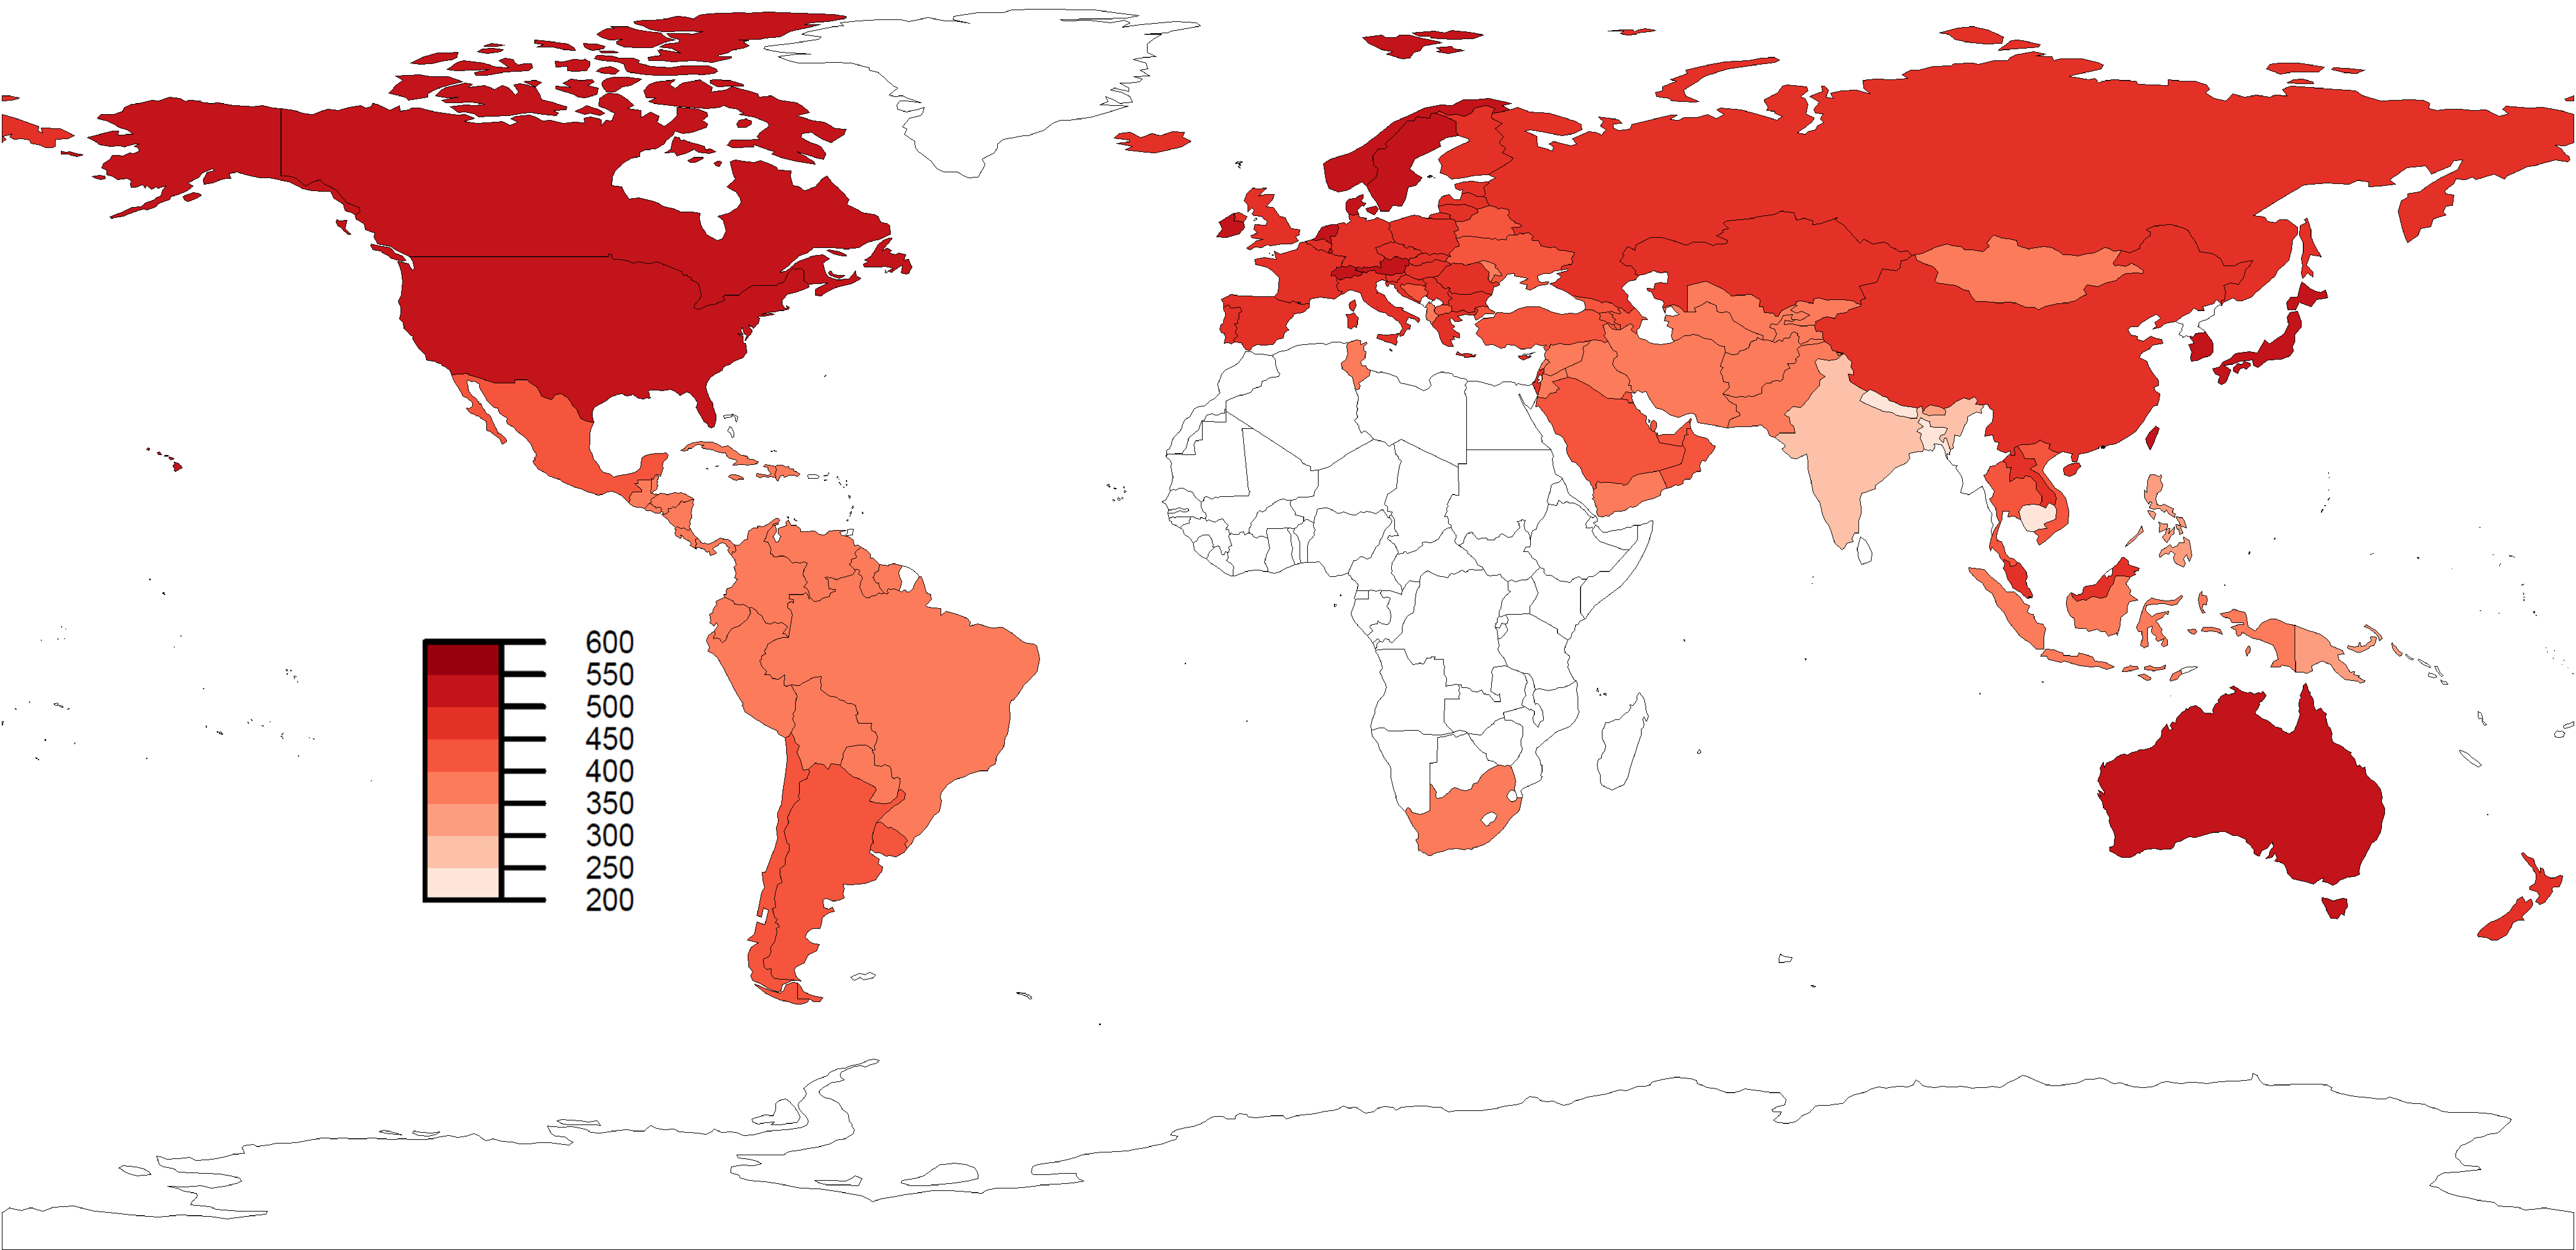
\includegraphics[width=.45\colwidmiddle]{PrS_LegendE.pdf}
  %     \caption{A map depicting the fitted (for countries in the dataset) \\* and predicted (for countries not in the dataset) test scores for \\* each country. A dark color represents a high score}
  %   \end{figure}
  % \end{minipage}

  \end{alertblock}
  \vskip2ex
\end{column}\begin{column}{\sepwid}\end{column}







\begin{column}{\colwidside}
% New column & block: Model selection
\begin{block}{Results}

  \vspace{.2in}
    \begin{minipage}[t]{0.45\linewidth}
    \begin{itemize} 
      \item \emph{Fitted} is based off our model fit, for the precincts included.
      \item \emph{Data} is based off the true data, for the precincts
        included.
      \item \emph{Reality} shows the actual observed election counts.
    \end{itemize}
  \end{minipage}
  \hfill
  \begin{minipage}[t]{0.75\linewidth}
    \centering
    \vspace{-1.5ex} 
    \begin{figure}
    \centering
      \begin{tabular}{r|c|c|c}
  Year & Fitted & Data & Reality \\
  \hline
  2002  & 6 & 6 & 6 \\
  2004  & 6 & 6 & 6 \\
  2006  & 6 & 7 & 7 \\ 
  2008  & 7 & 8 & 8 \\
  2010  & 4 & 8 & 7 \\
  2012  & 3 & 3 & 4 \\
  2014  & 3 & 3 & 3 \\
  2016  & 4 & 3 & 3 \\
  \hline      
  2018  & 3 & 4 & 2 or 3 \\
\end{tabular}

    \caption{Total Democratic District Winners}
    \end{figure}
  \end{minipage} 



  
% Below a graph depicting the model selection process is given. 
%   \begin{figure}[ht]
%     \centering
%       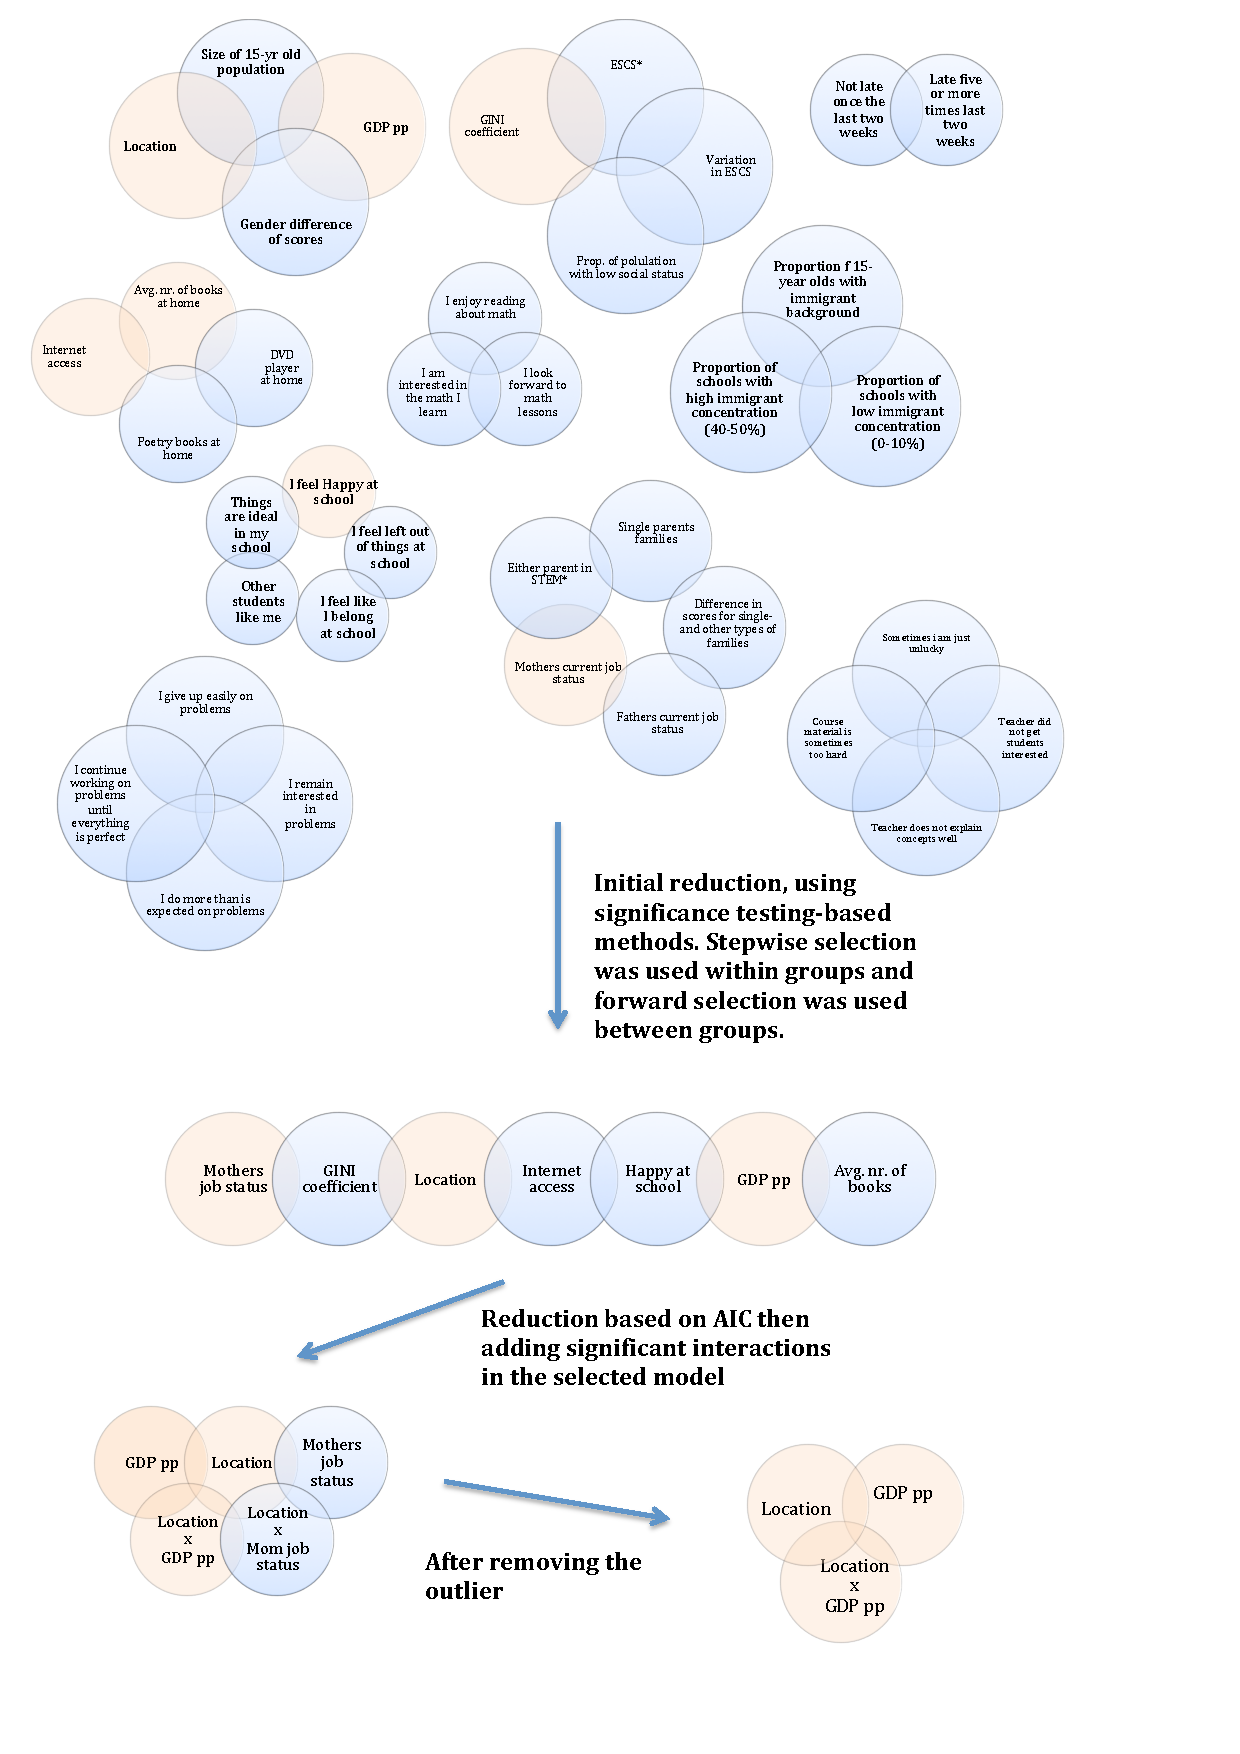
\includegraphics[width=.55\colwidmiddle]{modelSelectionGraph-1stpage.pdf}
%     \caption{Each circle represents a factor that was examined. The reduction was performed in three steps, denoted by arrows. The red circles represent factors which we chose to keep, and the blue circles represent factors which we chose to remove after the respective reductions.}
%   \end{figure}

\end{block}
   \vskip2ex

   
 \vspace{8in}
 \begin{block}{Conclusions}
\begin{itemize}
  \item Because of Gerrymandering -- the final vote results are
    surprisingly invariant to precinct level voting changes.
  \item As expected, the $\beta$ values 
\end{itemize}   
 \end{block}
   \vskip2ex
 
\end{column}

\begin{column}{\sepwid}\end{column}
\end{columns}
\end{frame}
\end{document}
